\documentclass[11pt]{article}
\usepackage[margin=1.2in]{geometry}
\usepackage{graphicx}
\usepackage{fancyhdr}
\usepackage{nopageno}%removes number on titlepage
\usepackage[parfill]{parskip}%adds lines in between paragraphs and takes out indentation
%\usepackage{subfig}
%\usepackage{multirow}
\usepackage{caption}
\usepackage{subcaption}

\begin{document}
% Cover page
\author{Chelsey Legacy, Lindong Zhou, Evan Pete Walsh\footnote{Statistics graduate students at Iowa State University of Science and Technology}}
\title{STAT 579 Final Project}
\maketitle

\begin{abstract}
Analysis of the Yelp Academic Dataset.
\end{abstract}

\newpage

\tableofcontents

\newpage

\pagenumbering{arabic}%starts numbering at "1"
\pagestyle{fancy}
\fancyhead[L]{Iowa State University}
\rhead{\thepage}
\rfoot{\today}
\cfoot{}%removes default page number at bottom center


\section{Introduction}

Lindong


\section{Data}

The Yelp Academic Dataset\footnote{$https://www.yelp.com/academic\_dataset$} provides data enthusiants with the exciting opportunity to explore an incredible collection of information regarding the characteristics and quality of hundreds of businesses across the United States, Canada, and the UK. Specifically, the data includes details and reviews on 250 of the closest businesses to 30 large universities, including the Arizona State, UNLV, the University of Edinburgh, the University of Wisconsin, and the University of Waterloo, to name a few. The raw data is in json format and contains five different types of json objects: \textbf{Business}, \textbf{Review}, \textbf{User}, \textbf{Check-in}, and \textbf{Tip}.

Each \textbf{Review} object represents an individual user-based review of a particular business. The unique encrypted business ID is given along with the date of the review, the number of stars (out of 5) that were awarded, the number and type of votes that the review received, and an optional text description provided by the user. \textbf{User} objects are unique to every person that has an active Yelp account. Each user has a name, a unique encrypted user ID, the number of votes they have cast, the average number of stars they have given, and the date they signed up for Yelp, among other things. A \textbf{Check-in} object represents the count and time of all the registered check-ins for a particular business, and \textbf{Tip} objects represent a tip given by user for a particular business. Tips include the user's ID, the business's ID, the date, and the message that the user gave. While these objects all provide a rich source of information, for the scope of this paper we will only be examing the \textbf{Business} objects.

\textbf{Business} objects are unique to business ID's, and include the following information:
\begin{itemize}
	\item the name of the business,
	\item the name of neighborhood in which the business is located,
	\item the city in which the business is located,
	\item the full address of the business,
	\item the exact latidude and longitude coordinates of the business,
	\item the average number of stars awarded to the business,
	\item the number of reviews received by the business,
	\item whether or not the business is still open,
	\item the hours that the business is open,
	\item the categories that the business falls under,
	\item and a number of different attributes which mostly concern restaurants and bars, such as whether or not smoking is allowed and the price range of the food.
\end{itemize}

To work with the data, we converted the set of all \textbf{Business} objects to a csv file in which the columns are variable names representing each aspect of a \textbf{Business} object, and each row corresponds to a unique business. Each different type of attribute was converted to its own character, numerical, or logical variable depending on what was appropriate. For example, the attribute \textbf{smoking} was converted to a logical variable where the value is ``true" if the smoking is allowed at the establishment, and ``false" if it is not allowed, while the attribute \textbf{price range} was converted to a numerical variable which ranges from 1 to 4.

\section{Restaurants}

Most of the data about restaurants in the Yelp Academic Dataset are concentrated around the following cities:
\begin{itemize}
	\item Madison, WI, 
	\item Las Vegas, NV,
	\item Pheonix, AZ,
	\item Waterloo, Ontario, Canada,
	\item and Edinburgh, Scotland.
\end{itemize}
Although the choice of cities is limited, the wealth of information coming from each city is abundant. All together, our data consists of 14,303 restaurants with 45 variables describing their attributes and the collective user sentiment towards each establishment. There is a significant number of restaurants in just about any subcategory that one can imagine. For example, Figure~\ref{fig:food01a} shows all of the restaurants classified as either ``hipster" or ``divey" near Pheonix, AZ that have telivisions, offer live music, and have more than 35 reviews on Yelp. Figure~\ref{fig:food01b} shows all of the Asian and Indian food restaurants near Las Vegas, NV that offer take-out and have a full bar.

\begin{figure}[h]
\caption{Restaurant subsets near Pheonix, AZ and Las Vegas, NV\label{fig:food01}}
\centering
\begin{subfigure}{0.45\linewidth}
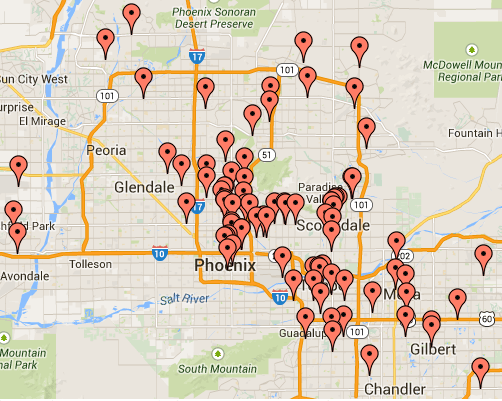
\includegraphics[width=\linewidth]{Figures/food_AZ.png}
\caption{All restaurants near Pheonix, AZ classified as ``hipster" or ``divey" that have live music, TV's, and more than 35 reviews on Yelp.}
\label{fig:food01a}
\end{subfigure}
\begin{subfigure}{0.45\linewidth}
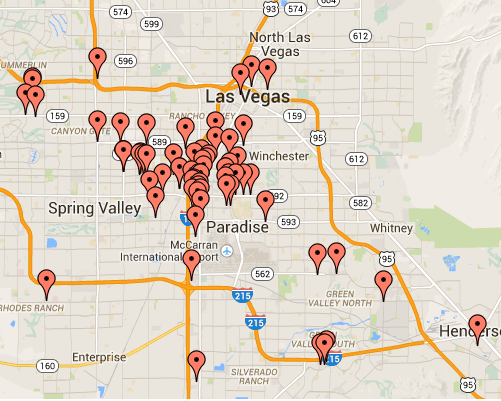
\includegraphics[width=\linewidth]{Figures/food_NV.png}
\caption{All Asian and Indian food restaurants near Las Vegas, NV that offer take-out and have a full bar.}
\label{fig:food01b}
\end{subfigure}
\end{figure}



\section{Bars}

The Business dataset contains a lot of information that can be used to analyze the relationship between different aspects of bar culture.  In order to analyze the bars available in the dataset, the data was subset to get rid of any businesses that did not have a full bar.  Looking at only the businesses with a full bar gives us insight into locations that serve from a full bar such as clubs, hotels, select restaurants, lounges, bowling alleys, and other various entertainment locations.  Through analyzing this data we can explore what attributes are likely to get a bar higher rating, what features bars most commonly share, and if lower ratings indicate a bar   
could shut down.

\subsection{Food}

\begin{figure}[h!]
  \caption{Plot of the number of stars a restaurant received filled with the type of food served at the bar.}
  \centering
  \label{food}
    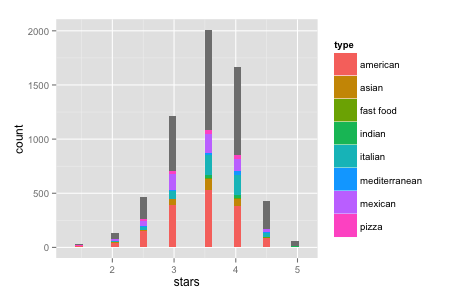
\includegraphics[width=0.5\textwidth]{Food_bars.png}
\end{figure}

Though not all bars serve food, many bars in restaurants do which begs the question; what is the most common food served in bars?  In order to investigate this question a qplot of the number of starts given to each bar filled with a count of the food types for each different rating will give us the information and more.  This data revealed unsurprisingly that the most common food served in American bars is American food (burgers, fries, etc). Through further analysis it is determined that 50$\%$ of the bars served primarily American style food.  We can see that the majority of each bar of star, no matter what the rating, is colored for American food.  However, looking more closely at the graph we can see that there is some unexpected information.  From Figure~\ref{food} we can see that there are a wide number of food options for people looking for full bars.  Along with American, Italian and Mexican are also abundant options making up 16$\%$ and 16.7$\%$ respectively.  Another piece of information we can infer from this graphic is that along with the plot of the stars a bar receives being a normal distribution, there also is a consistency in the number of each type of food being represented at each level of stars a bar receives.  Thus, we can see there is no preference for food when looking for a certain quality bar. A bar is equally likely to serve American food whether it receives 1 star or 5 stars.  In order to investigate this I ran more analysis.  





\section{Hotels}

Lindong

\section{Fitness}

Lindong


\section{Conclusion}


Chelsey




\end{document}